\section{Background}
\label{sec:background}

We provide some background on the performance characteristics and execution
model of GPUs.
We also describe the standard implementation of attention, as well as
\sysnameone.

\subsection{Hardware characteristics}
\label{subsec:hardware}

\textbf{GPU performance characteristics.}
The GPU consists of compute elements (e.g., floating point arithmetic units) and
a memory hierarchy.
Most modern GPUs contain specialized units to accelerate matrix multiply in
low-precision (e.g., Tensor Cores on Nvidia GPUs for FP16/BF16 matrix multiply).
The memory hierarchy comprise of high bandwidth memory (HBM), and on-chip SRAM
(aka shared memory).
As an example, the A100 GPU has 40-80GB of high bandwidth memory (HBM) with
bandwidth 1.5-2.0TB/s and 192KB of on-chip SRAM per each of 108 streaming
multiprocessors with bandwidth estimated around 19TB/s~\citep{jia2018dissecting,
  jia2021dissecting}.
As the L2 cache is not directly controllable by the programmer, we focus on the
HBM and SRAM for the purpose of this discussion.
% The on-chip SRAM is an order of magnitude faster than HBM but many orders of
% magnitude smaller in size.
% As specialized computation (matrix multiply) has gotten faster relative to memory
% speed~\citep{nvidia2017nvidia,nvidia2020nvidia,nvidia2022nvidia},
% operations are increasingly bottlenecked by memory (HBM) accesses.
% Thus exploiting fast SRAM becomes more important.

\textbf{Execution Model.}
GPUs have a massive number of threads to execute an operation
(called a kernel).
Threads are organized into thread blocks, which are scheduled to run on
streaming multiprocessors (SMs).
Within each thread blocks, threads are grouped into warps (a group of 32
threads).
Threads within a warp can communicate by fast shuffle instructions or cooperate
to perform matrix multiply.
Warps within a thread block can communicate by reading from / writing to shared memory.
Each kernel loads inputs from HBM to registers and SRAM, computes, then writes outputs to HBM.

\subsection{Standard Attention Implementation}
\label{subsec:standard_attn}

Given input sequences $\vQ, \vK, \vV \in \mathbb{R}^{N \times d}$ where $N$ is the sequence length and
$d$ is the head dimension, we want to compute the attention output $\vO \in \mathbb{R}^{N \times d}$:
\begin{equation*}
  \vS = \vQ \vK^\top \in \mathbb{R}^{N \times N}, \quad \vP = \softmax(\vS) \in \mathbb{R}^{N \times N}, \quad \vO = \vP\vV \in \mathbb{R}^{N \times d},
\end{equation*}
where $\softmax$ is applied row-wise.\footnote{For clarity of exposition, we
  omit the scaling of $\vQ \vK^\top$ (typically by $1/\mathrm{d}$), and optionally
  elementwise masking on $\vS$ and/or dropout applied to $\vP$} For multi-head
attention (MHA), this same computation is performed in parallel across many
heads, and parallel over the batch dimension (number of input sequences in a
batch).

The backward pass of attention proceeds as follows.
Let $\vdO \in \mathbb{R}^{N \times d}$ be the gradient of $\vO$ with respect to some loss
function. Then by the chain rule (aka backpropagation):
\begin{align*}
  \vdV &= \vP^\top \vdO \in \mathbb{R}^{N \times d} \\
  \vdP &= \vdO \vV^\top \in \mathbb{R}^{N \times N} \\
  \vdS &= \dsoftmax (\vdP) \in \mathbb{R}^{N \times N} \\
  \vdQ &= \vdS \vK \in \mathbb{R}^{N \times d} \\
  \vdK &= \vQ \vdS^\top \in \mathbb{R}^{N \times d},
\end{align*}
where $\dsoftmax$ is the gradient (backward pass) of softmax applied row-wise.
One can work out that if $p = \softmax(s)$ for some vector $s$ and $p$, then
with output gradient $dp$, the input gradient $ds = (\diag(p) - p p^\top)dp$.

Standard attention implementations materialize the matrices $\vS$ and $\vP$ to
HBM, which takes $O(N^2)$ memory.
Often $N \gg d$ (typically $N$ is on the order of 1k--8k and $d$ is around 64--128).
The standard attention implementation (1) calls the matrix multiply (GEMM)
subroutine to multiply $\vS = \vQ \vK^\top$, writes the result to HBM, then (2)
loads $\S$ from HBM to compute softmax and write the result $\vP$ to HBM, and
finally (3) calls GEMM to get $\vO = \vP \vV$.
As most of the operations are bounded by memory bandwidth, the large number of
memory accesses translates to slow wall-clock time.
Moreover, the required memory is $O(N^2)$ due to having to materialize $\vS$ and
$\vP$.
Moreover, one has to save $\vP \in \mathbb{R}^{N \times N}$ for the backward pass to compute the
gradients.

\subsection{\sysnameone}
\label{subsec:flashv1}

To speed up attention on hardware accelerators such as GPU,
\citep{dao2022flashattention} proposes an algorithm to reduce the memory
reads/writes while maintaining the same output (without approximation).

\subsubsection{Forward pass}
\sysnameone applies the classical technique of tiling to reduce memory IOs, by
(1) loading blocks of inputs from HBM to SRAM, (2) computing attention with
respect to that block, and then (3) updating the output without writing the
large intermediate matrices $\vS$ and $\vP$ to HBM.
As the softmax couples entire rows or blocks of row, online
softmax~\citep{milakov2018online, rabe2021self} can split the attention
computation into blocks, and rescale the output of each block to finally get the
right result (with no approximation).
By significantly reducing the amount of memory reads/writes, \sysnameone yields
2-4$\times$ wall-clock speedup over optimized baseline attention implementations.

We describe the online softmax technique~\citep{milakov2018online} and how it is
used in attention~\citep{rabe2021self}.
For simplicity, consider just one row block of the attention matrix $\vS$, of the form
$\begin{bmatrix} \vS^{(1)} & \vS^{(2)} \end{bmatrix}$ for some matrices
$\vS^{(1)}, \vS^{(2)} \in \mathbb{R}^{B_r \times B_c}$, where $B_r$ and $B_c$ are the row and
column block sizes.
We want to compute softmax of this row block and multiply with the value,
of the form $\begin{bmatrix} \vV^{(1)} \\ \vV^{(2)} \end{bmatrix}$ for some
matrices $\vV^{(1)}, \vV^{(2)} \in \mathbb{R}^{B_c \times d}$.
Standard softmax would compute:
\begin{align*}
  m &= \max(\mathrm{rowmax}(\vS^{(1)}), \mathrm{rowmax}(\vS^{(2)})) \in \mathbb{R}^{B_r}  \\
  \ell &= \mathrm{rowsum}(e^{\vS^{(1)} - m}) + \mathrm{rowsum}(e^{\vS^{(2)} - m}) \in \mathbb{R}^{B_r}  \\
  \vP &= \begin{bmatrix} \vP^{(1)} & \vP^{(2)} \end{bmatrix} = \diag(\ell)^{-1}\begin{bmatrix} e^{\vS^{(1)} - m} & e^{\vS^{(2)} - m} \end{bmatrix} \in \mathbb{R}^{B_r \times 2B_c} \\
  \vO &= \begin{bmatrix} \vP^{(1)} & \vP^{(2)} \end{bmatrix} \begin{bmatrix} \vV^{(1)} \\ \vV^{(2)} \end{bmatrix} = \diag(\ell)^{-1} e^{\vS^{(1)} - m} \vV^{(1)} + e^{\vS^{(2)} - m} \vV^{(2)} \in \mathbb{R}^{B_r \times d}.
\end{align*}
Online softmax instead computes ``local'' softmax with respect to each block and
rescale to get the right output at the end:
\begin{align*}
  m^{(1)} &= \mathrm{rowmax}(\vS^{(1)})  \in \mathbb{R}^{B_r}\\
  \ell^{(1)} &= \mathrm{rowsum}(e^{\vS^{(1)} - m^{(1)}}) \in \mathbb{R}^{B_r} \\
  \tilde{\vP}^{(1)} &= \diag(\ell^{(1)})^{-1} e^{\vS^{(1)} - m^{(1)}} \in \mathbb{R}^{B_r \times B_c}\\
  \vO^{(1)} &= \tilde{\vP}^{(1)} \vV^{(1)} = \diag(\ell^{(1)})^{-1} e^{\vS^{(1)} - m^{(1)}} \vV^{(1)} \in \mathbb{R}^{B_r \times d}\\
  m^{(2)} &= \max(m^{(1)}, \mathrm{rowmax}(\vS^{(2)})) = m \\
  \ell^{(2)} &= e^{m^{(1)} - m^{(2)}} \ell^{(1)} + \mathrm{rowsum}(e^{\vS^{(2)} - m^{(2)}}) = \mathrm{rowsum}(e^{\vS^{(1)} - m}) + \mathrm{rowsum}(e^{\vS^{(2)} - m}) = \ell \\
  \tilde{\vP}^{(2)} &= \diag(\ell^{(2)})^{-1} e^{\vS^{(2)} - m^{(2)}} \\
  \vO^{(2)} &= \diag(\ell^{(1)} / \ell^{(2)})^{-1} \vO^{(1)} + \tilde{\vP}^{(2)} \vV^{(2)} = \diag(\ell^{(2)})^{-1} e^{s^{(1)} - m} \vV^{(1)} + \diag(\ell^{(2)})^{-1} e^{s^{(2)} - m} \vV^{(2)} = \vO.
\end{align*}

We show how \sysnameone uses online softmax to enable tiling
(\cref{fig:flash_attention_diagram}) to reduce memory reads/writes.
\begin{figure}[ht]
  \centering
  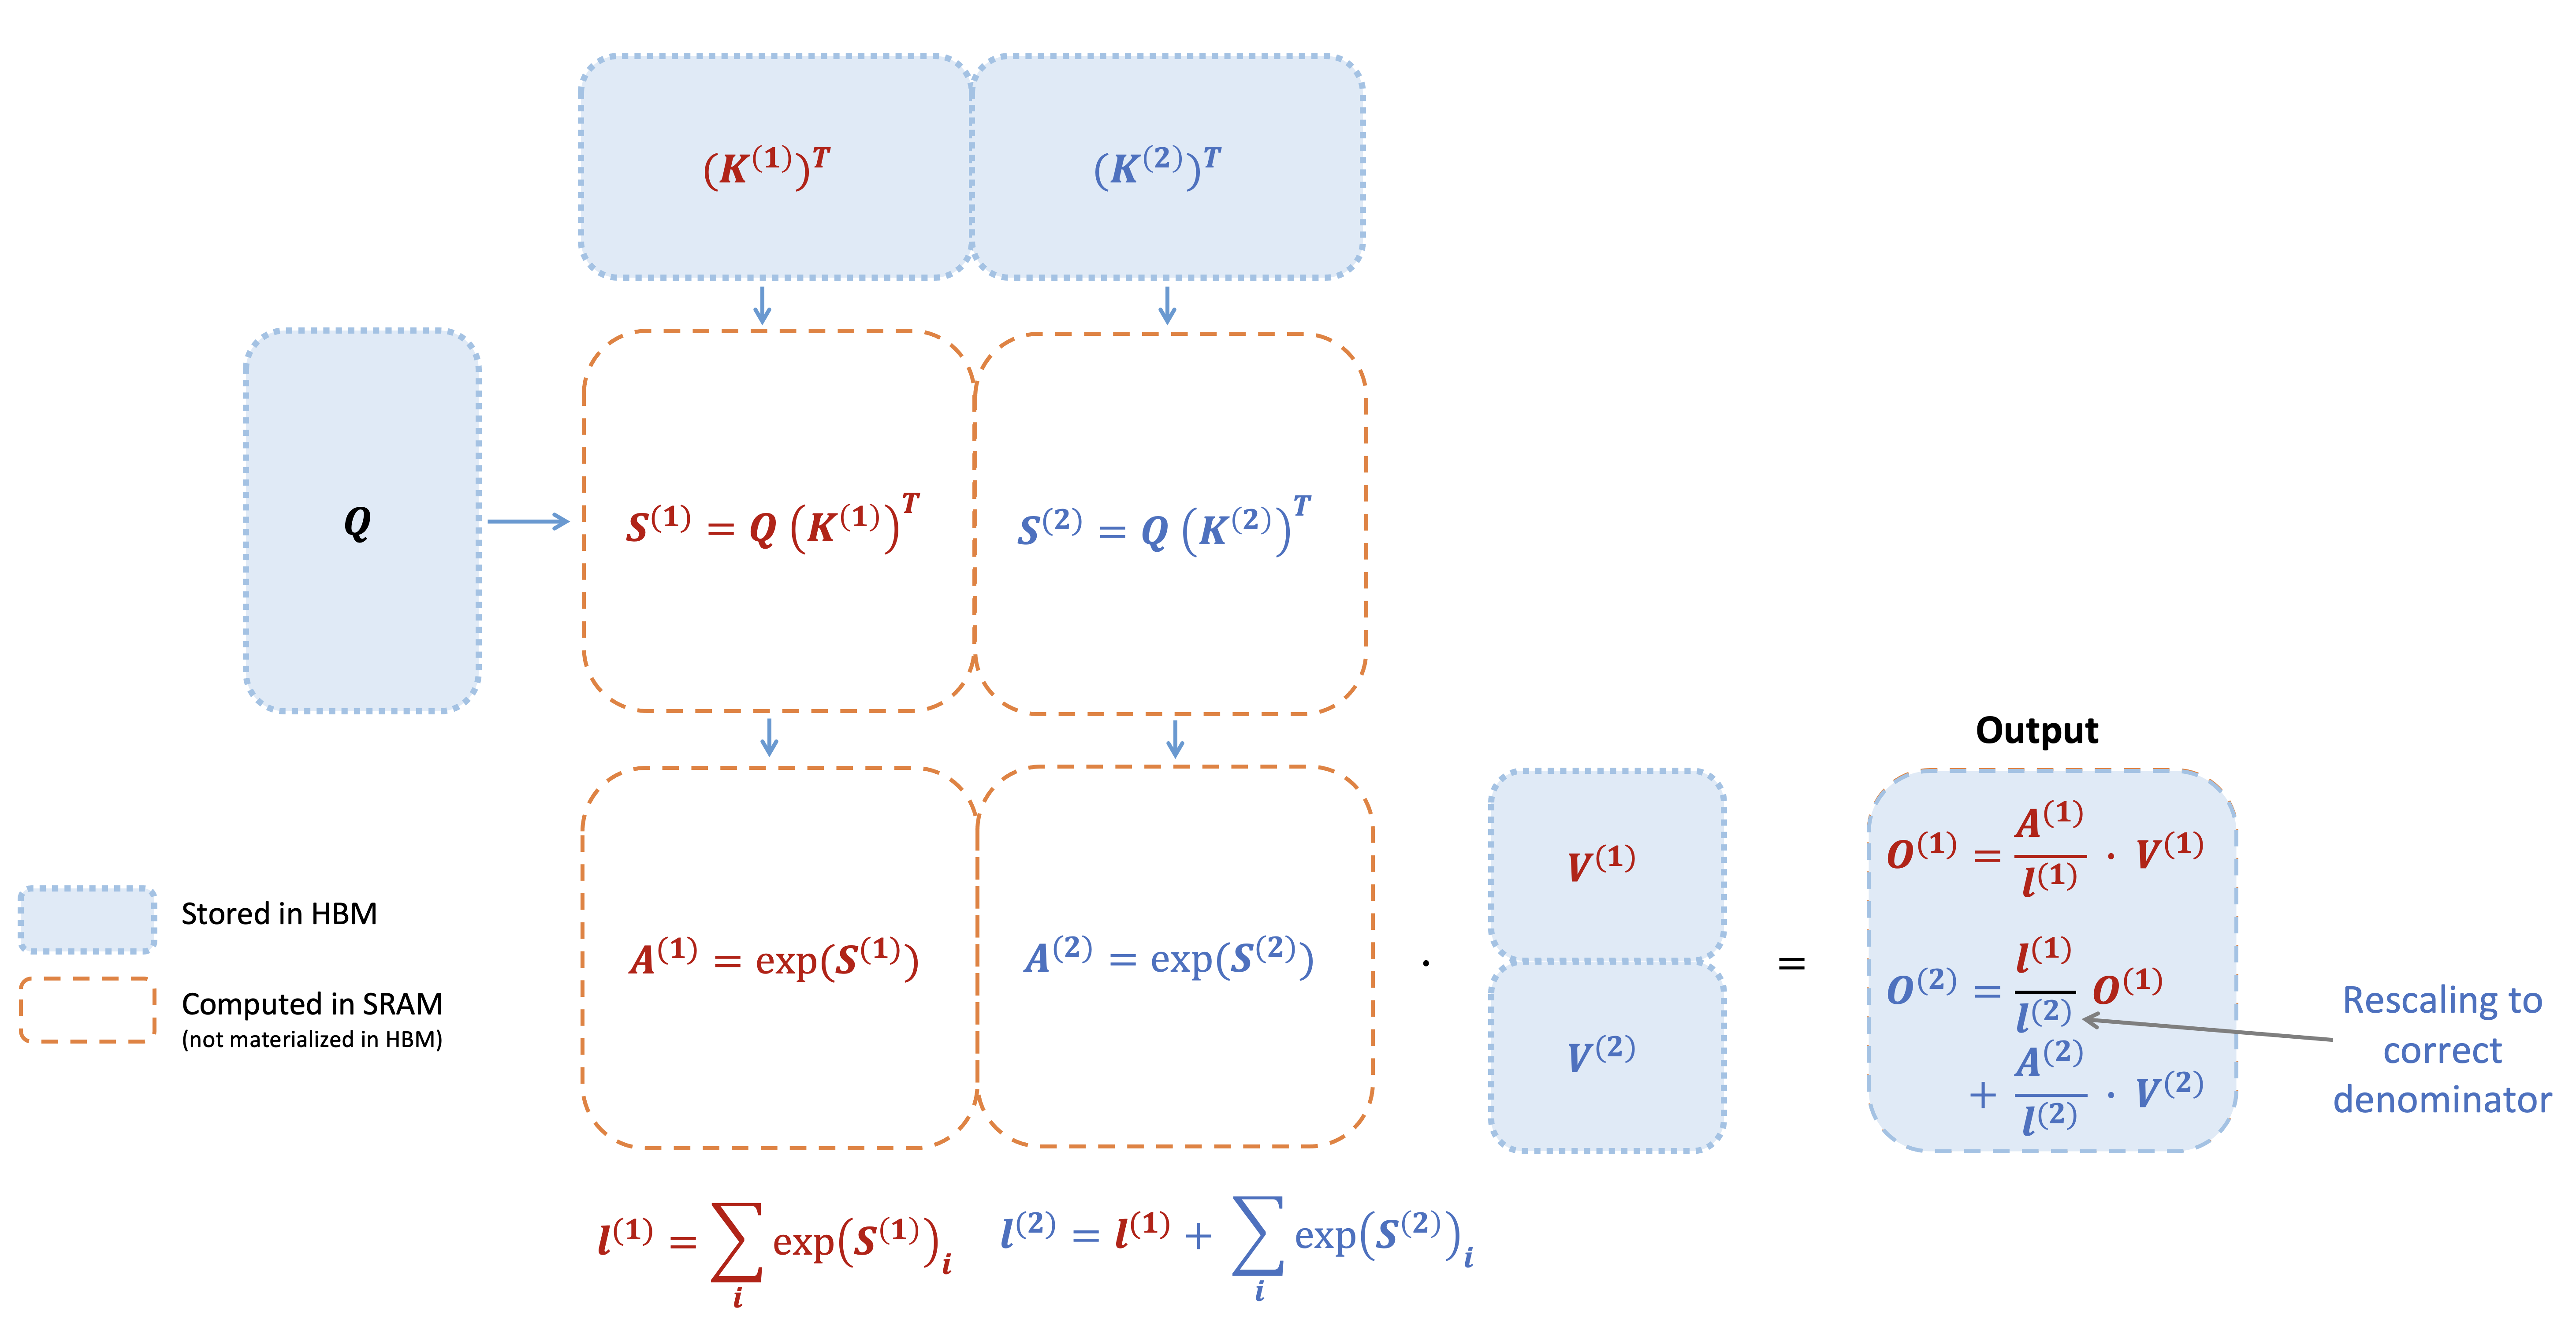
\includegraphics[width=0.9\textwidth]{figs/flash_attention_diagram.png}
  \caption{\label{fig:flash_attention_diagram}Diagram of how \sysnameone forward
    pass is performed, when the key $\vK$ is partitioned into two blocks and the
    value $\vV$ is also partitioned into two blocks.
    By computing attention with respect to each block and rescaling the output,
    we get the right answer at the end, while avoiding expensive memory
    reads/writes of the intermediate matrices $\vS$ and $\vP$.
    We simplify the diagram, omitting the step in softmax that subtracts each
    element by the row-wise max.}
\end{figure}

\subsubsection{Backward pass}
In the backward pass, by re-computing the values of the attention matrices $\vS$
and $\vP$ once blocks of inputs $\vQ, \vK, \vV$ are already loaded to SRAM,
\sysnameone avoids having to store large intermediate values.
By not having to save the large matrices $\vS$ and $\vP$ of size $N \times N$,
\sysnameone yields 10-20$\times$ memory saving depending on sequence length (memory
required in linear in sequence length $N$ instead of quadratic).
The backward pass also achieves 2-4$\times$ wall-clock speedup due to reduce memory
reads/writes.

The backward pass applies tiling to the equations in~\cref{subsec:standard_attn}.
Though the backward pass is simpler than the forward pass conceptually (there is
no softmax rescaling), the implementation is significantly more involved.
This is because there are more values to be kept in SRAM to perform 5 matrix
multiples in the backward pass, compared to just 2 matrix multiples in the
forward pass.

%%% Local Variables:
%%% mode: latex
%%% TeX-master: "../flash2"
%%% End:
